\documentclass[paper=a4,oneside,fontsize=12pt,DIV=14,headings=normal,parskip=half,headsepline,numbers=noendperiod]{scrreprt}
\usepackage[T1]{fontenc}
\usepackage[utf8]{inputenc}
\usepackage[english]{babel}
\usepackage{lmodern}
\usepackage[bitstream-charter]{mathdesign}
\usepackage[scaled=0.92]{helvet}
\usepackage{microtype}
\usepackage[onehalfspacing]{setspace}
\usepackage[outer=25mm,inner=30mm,top=26mm,bottom=28mm,heightrounded=true]{geometry}
\usepackage{mathtools,bm}
\usepackage{amsthm}
\usepackage{booktabs,tabularx,array}
\usepackage{enumitem}
\usepackage{xcolor}
\usepackage{graphicx}
\usepackage{float}
\usepackage[automark]{scrlayer-scrpage}
\usepackage[hidelinks]{hyperref}
\usepackage[nameinlink,noabbrev]{cleveref}
\setcounter{secnumdepth}{3}
\setcounter{tocdepth}{2}
\addtokomafont{disposition}{\normalfont\bfseries}
\setkomafont{pageheadfoot}{\normalfont\small}
\ihead{Embedded-Penalty SDA Analysis}
\chead{}
\ohead{\pagemark}
\cfoot{}
\setlength{\emergencystretch}{2em}
\renewcommand{\arraystretch}{1.18}
\newcommand{\vct}[1]{\bm{#1}}
\newcommand{\mat}[1]{\bm{#1}}
\newcommand{\T}{\mathsf{T}}
\newcommand{\norm}[1]{\left\lVert#1\right\rVert}
\newtheorem{proposition}{Proposition}[chapter]
\newtheorem{corollary}{Corollary}[chapter]

\begin{document}
\begin{titlepage}
\centering
\vspace*{3.0cm}
{\sffamily\bfseries\fontsize{23}{28}\selectfont
Hybrid Sphere Decoding with Embedded Initialization and Explicit Pruning\par}
\vspace{0.55cm}
{\sffamily\fontsize{16}{20}\selectfont
A paired study of leaf-cost equivalence, partial metrics, pruning margins,
and sphere-decoder search paths\par}
\vspace{1.2cm}
{\sffamily\bfseries\fontsize{15}{18}\selectfont Thesis Analysis Note\par}
\vfill
\begin{minipage}{0.84\textwidth}
\small
This document develops the argument for a hybrid sphere decoder that uses the
embedded zero-vector formulation to construct its initial incumbent and the
explicit formulation to perform exact branch-and-bound enumeration.  The
argument is organized around leaf-level objective equivalence, upper-bound
quality, prefix-bound tightness, and a controlled ablation study.  Its purpose
is to provide a rigorous source for later integration into the master thesis.
\end{minipage}
\vfill
{\large October 2026\par}
\end{titlepage}
\pagenumbering{roman}
\tableofcontents
\clearpage
\pagenumbering{arabic}

\chapter{Terminology and How to Read the Diagnostics}
\label{chap:terminology}

This chapter defines the search-specific terms used in the report.  They are
introduced here because several familiar statistical words have a precise
meaning in the present SDA experiment.

\section{Search tree, node, depth, prefix, and leaf}
A \emph{search tree} is a representation of all binary switching sequences.
At each level, the search chooses either zero or one for the next element of
$\vct U$.  A \emph{node} is one such attempted choice together with the choices
already made before it.  Visiting a node means that the solver has formed this
partial candidate and calculated its partial metric; it does not mean that the
candidate is accepted or optimal.

The \emph{depth} $i$ is the number of binary variables currently fixed.  The
implemented forward search begins at $i=1$ and ends at $i=15$.  The vector of
the first $i$ fixed decisions is called a \emph{prefix}, or partial switching
sequence:
\begin{equation}
 \vct U_{1:i}=[U_1,U_2,\ldots,U_i]^\T.
\end{equation}
For example, if a complete candidate begins with
\begin{equation}
 \vct U=[0,0,1,\;1,0,1,\ldots]^\T,
\end{equation}
then its prefixes at depths 1, 3, and 6 are $0$, $001$, and $001101$,
respectively.  A depth-three prefix is the first complete three-phase switching
vector.  Complete switching-vector boundaries therefore occur at
$i=3,6,9,12,15$.  At depth $i$ there are $2^i$ possible prefixes.

A \emph{leaf} is a node at depth 15, where every element of $\vct U$ is known.
Only a leaf represents a complete admissible switching sequence and has a full
objective value.  An internal node represents only a prefix and is evaluated
using a lower, partial cost.

\section{Partial metric, incumbent, radius, and pruning}
The \emph{partial metric} $P_i$ is the cost accumulated from the information
available at depth $i$.  It is a lower bound used to decide whether completing
the prefix can still be worthwhile.  It is not generally the final physical
cost of a switching sequence.

The best complete sequence found so far is the \emph{incumbent}.  Its cost is
the current \emph{sphere radius} $R$.  ``Radius'' is inherited from the
geometric interpretation of sphere decoding; in the program, it is a scalar
cost threshold rather than a physical length.  The initial incumbent is
provided by the best of the Round, Shift, and Babai candidates.  Whenever the
search finds a better leaf, that leaf becomes the new incumbent and $R$
decreases.  The term \emph{dynamic radius} emphasizes that $R$ can change many
times during one SDA call.

\emph{Pruning} means terminating a branch because its partial metric already
exceeds the incumbent:
\begin{equation}
 P_i>R.
\end{equation}
The descendants of that prefix are then not visited.  A \emph{surviving node}
is a tested node with $P_i\leq R$ that may be expanded to the next depth.

The \emph{pruning margin} is
\begin{equation}
 M_i=R-P_i.
\end{equation}
It can be read as the remaining cost allowance of the tested prefix:
\begin{itemize}
 \item $M_i>0$: the prefix is still inside the current sphere and survives;
 \item $M_i=0$: the prefix lies on the pruning boundary;
 \item $M_i<0$: the prefix is outside the sphere and is pruned.
\end{itemize}
A large positive margin does not mean that the prefix is close to optimal.  It
only means that the available lower bound is not yet large enough to reject it.

\section{Paired observation and paired node-count difference}
Two observations are \emph{paired} when they describe the same operating
condition and the same controller transaction.  Thus, the embedded and
explicit node counts at time $t_k$ form one pair.  The paired node-count
difference is
\begin{equation}
 \Delta N_k=N_{\mathrm{emb},k}-N_{\mathrm{exp},k}.
\end{equation}
A positive value means that the embedded formulation visited more nodes for
that same physical case.  Pairing prevents a heavily loaded embedded sample
from being compared accidentally with a lightly loaded explicit sample.

\section{Probability density and kernel-density estimate}
A histogram divides node differences into bins.  A \emph{kernel-density
estimate} (KDE) is a smooth version of the same distribution.  Each measured
$\Delta N_k$ contributes a small smooth kernel, and their sum forms the plotted
curve.  The vertical axis is \emph{probability density}, not the probability of
one exact node difference.  The area under the complete curve equals one:
\begin{equation}
 \int_{-\infty}^{\infty}\widehat f_h(x)\,\mathrm dx=1.
\end{equation}
The probability that $\Delta N$ lies in an interval is the area under the curve
over that interval.  Consequently, a vertical value such as
$1.4\times10^{-3}$ should not be interpreted as $0.14\%$ of the samples.  Its
unit is approximately inverse nodes, and it becomes a probability only after
integration over a node-count interval.

\section{Median, quartiles, IQR, and representative percentiles}
The \emph{median}, also denoted $Q_{50}$, is the value below which half the
observations lie.  The first and third quartiles, $Q_{25}$ and $Q_{75}$,
enclose the middle half of the observations.  The \emph{interquartile range}
(IQR) is the interval
\begin{equation}
 \mathrm{IQR}=[Q_{25},Q_{75}].
\end{equation}
In the figures, a solid line commonly shows the median and a shaded band shows
the IQR.  A wide band indicates strong path-to-path variation.

The labels $Q_5$, $Q_{50}$, and $Q_{95}$ used for representative transactions
refer to percentiles of the paired node difference $\Delta N$: a weak
difference case, a typical case, and a pronounced difference case.  They do
not refer to motor torque, confidence intervals, or prediction horizons.

\section{Same-prefix comparison and initial-sphere membership}
The actual embedded and explicit searches visit different nodes in different
orders.  Their 100th visited nodes therefore need not represent the same
partial switching sequence.  A \emph{same-prefix comparison} instead fixes one
specific pair $(i,\vct U_{1:i})$ and evaluates that identical prefix under both
cost representations.  Enumerating all $2^i$ prefixes at each depth produces a
comparison that is independent of the actual traversal order.

A prefix is described as \emph{inside the initial sphere} when its partial
metric does not exceed the radius before any search-generated radius update:
\begin{equation}
 P_i\leq R_0.
\end{equation}
This is a static diagnostic.  It does not predict the complete real search on
its own because the actual radius may shrink after an improved leaf is found.

\section{Effective offset and representation-induced prefix slack}
For an identical prefix, the effective accumulated difference is
\begin{equation}
 C_i^{\mathrm{eff}}=P_i^{\mathrm{emb}}-P_i^{\mathrm{exp}}.
\end{equation}
It answers: ``At this depth, how much more partial metric has the embedded
representation accumulated for the same binary choices?''  The
representation-induced prefix slack is
\begin{equation}
 S_i=6250-C_i^{\mathrm{eff}}.
\end{equation}
A positive $S_i$ means that the full leaf offset 6250 has not yet appeared in
the difference between the two partial metrics.  It does not automatically
mean that the embedded node survives, because each formulation can have a
different and dynamically changing radius.

\chapter{Problem Statement and Experimental Observation}

The long-horizon finite-control-set model predictive controller uses a binary
sphere decoder to determine a switching sequence
\begin{equation}
 \vct U=[S_{a,1},S_{b,1},S_{c,1},\ldots,S_{a,N_p},S_{b,N_p},S_{c,N_p}]^\T,
 \qquad \vct U\in\{0,1\}^{3N_p},
\end{equation}
with $N_p=5$ and hence 15 binary decision variables.  Two mathematically
equivalent treatments of the zero vectors $000$ and $111$ were implemented.
The first adds a discrete penalty when a complete three-switch block is known.
The second incorporates an equivalent quadratic expression into the Hessian
before its Cholesky factorization.

Paired simulations at 10, 50, and 90~Nm produced the following initially
surprising observations.
\begin{enumerate}
 \item The two formulations returned identical optimal switching sequences in
 all paired samples considered.
 \item The embedded formulation reported an optimal cost approximately 6250
 larger than the explicit formulation at every transaction.
 \item The embedded formulation visited substantially more search nodes.
 \item Babai initialization was the best of the tested initializers in both
 formulations and dominated especially strongly in the embedded formulation.
\end{enumerate}
These results separate control equivalence from computational equivalence.  An
identical minimizer at the leaves of a search tree does not imply identical
partial metrics or identical pruning decisions inside the tree.

\section{Central argument of the hybrid method}
The analysis is organized around three claims.
\begin{enumerate}
 \item The explicit and embedded objectives are equivalent on complete binary
 sequences up to a constant.  A feasible sequence obtained from one
 representation can therefore initialize the other without changing the
 optimizer.
 \item The embedded geometry includes the zero-vector preference when the
 Babai point is constructed and consequently provides a substantially better
 initial upper bound than the native explicit initializer in the investigated
 cases.
 \item The explicit formulation applies the exact penalty at complete
 three-switch block boundaries and supplies tighter normalized prefix bounds
 at these depths.  It therefore requires fewer nodes to certify optimality.
\end{enumerate}
The proposed hybrid uses the embedded formulation only for incumbent
generation and then evaluates that incumbent under the exact explicit
objective before commencing explicit SDA enumeration.

\chapter{Leaf-Level Equivalence of the Two Penalties}

\section{Exact binary representation}
For one three-phase switching vector define
\begin{equation}
 m=S_a+S_b+S_c,\qquad m\in\{0,1,2,3\}.
\end{equation}
The vector is a zero vector exactly when $m=0$ or $m=3$.  The explicit cost is
\begin{equation}
 J_{\mathrm{z,exp}}(m)=
 \begin{cases}
  \lambda_z,&m\in\{0,3\},\\
  0,&m\in\{1,2\}.
 \end{cases}
\end{equation}
On the binary domain this logic is represented exactly by
\begin{equation}
 J_{\mathrm{z,exp}}(m)
 =\frac{\lambda_z}{2}(m-1)(m-2).
\end{equation}
The centered quadratic used by the embedded formulation is
\begin{equation}
 J_{\mathrm{z,emb}}(m)=\frac{\lambda_z}{2}(m-1.5)^2.
\end{equation}
Consequently,
\begin{equation}
 \boxed{J_{\mathrm{z,emb}}(m)
 =J_{\mathrm{z,exp}}(m)+\frac{\lambda_z}{8}.}
 \label{eq:block_offset}
\end{equation}

For $\lambda_z=10{,}000$, the explicit costs of zero and active vectors are
$10{,}000$ and zero, whereas the embedded costs are $11{,}250$ and $1{,}250$.
Both therefore retain the same zero-to-active cost difference of $10{,}000$.
The embedded representation merely adds $1250$ to every complete switching
vector.  Over $N_p=5$ steps,
\begin{equation}
 C=\frac{N_p\lambda_z}{8}=6250.
 \label{eq:total_offset}
\end{equation}
For every complete binary sequence,
\begin{equation}
 J_{\mathrm{emb}}(\vct U)=J_{\mathrm{exp}}(\vct U)+C,
\end{equation}
and therefore both formulations have the same minimizer.

\begin{proposition}[Leaf-level objective equivalence]
For $\vct U\in\{0,1\}^{3N_p}$, the embedded and explicit objectives satisfy
\begin{equation}
 J_{\mathrm{emb}}(\vct U)
 =J_{\mathrm{exp}}(\vct U)+\frac{N_p\lambda_z}{8}.
\end{equation}
Consequently, their complete-sequence minimizer sets are identical.
\end{proposition}
\begin{proof}
Equation~\eqref{eq:block_offset} holds independently for every prediction
block.  Summing it over $N_p$ blocks produces a sequence-independent constant.
Adding a constant to all feasible objective values preserves every pairwise
ordering and therefore preserves the set of minimizers.
\end{proof}

\section{Why leaf equivalence does not prove search equivalence}
The SDA does not wait until all 15 variables are known.  With the lower
triangular factor used by the implemented forward search, its quadratic partial
metric at depth $i$ is
\begin{equation}
 P_i^{\mathrm{quad}}
 =\sum_{k=1}^{i}
 \left(
  (H U_{\mathrm{unc}})_k-
  \sum_{j=1}^{k}H_{kj}U_j
 \right)^2.
 \label{eq:quadratic_partial}
\end{equation}
A branch is pruned when its complete partial metric exceeds the current
incumbent radius $R$:
\begin{equation}
 P_i>R.
 \label{eq:prune_rule}
\end{equation}
Equation~\eqref{eq:total_offset} constrains the leaf cost at $i=15$, but it
does not imply that partial metrics at $i<15$ differ by a fixed or uniformly
distributed fraction of 6250.

\chapter{Search Mechanism and Working Hypotheses}

\section{Explicit block-boundary penalty}
The production search proceeds from $i=1$ to $i=15$.  At
$i=3,6,9,12,15$, a complete three-phase vector is available.  The explicit
formulation then evaluates the zero-vector condition and, if necessary, adds
$\lambda_z$ immediately.  This creates a semantic alignment between the
physical event ``a zero vector has been completed'' and a discrete jump in the
partial search metric.

\section{Embedded quadratic representation}
Using $S_x^2=S_x$ for binary variables, the embedded block cost expands to
\begin{equation}
 J_{\mathrm{z,emb}}
 =\frac{9\lambda_z}{8}
 -\lambda_z(S_a+S_b+S_c)
 +\lambda_z(S_aS_b+S_aS_c+S_bS_c).
\end{equation}
It is therefore not composed of three independent one-third penalties.  Its
final classification is produced jointly by linear and pairwise terms.  After
the complete Hessian is factorized,
\begin{equation}
 \mat W=\mat H\mat H^\T,
\end{equation}
the original block meaning is generally redistributed among several squared
residuals.  The individual residual increment at one search level is thus not
itself interpretable as a fraction of the zero-vector penalty.

\section{Refined prefix-slack hypothesis}
For the same binary prefix, define the effective accumulated difference
\begin{equation}
 C_i^{\mathrm{eff}}
 =P_i^{\mathrm{emb}}-P_i^{\mathrm{exp}}
 \label{eq:effective_offset}
\end{equation}
and the remaining representation-induced prefix slack
\begin{equation}
 S_i=C-C_i^{\mathrm{eff}}.
 \label{eq:prefix_slack}
\end{equation}
If the two initial radii differ by $C$, the pruning margins satisfy
\begin{align}
 M_i^{\mathrm{exp}}&=R_{\mathrm{exp}}-P_i^{\mathrm{exp}},\\
 M_i^{\mathrm{emb}}&=R_{\mathrm{emb}}-P_i^{\mathrm{emb}},\\
 M_i^{\mathrm{emb}}-M_i^{\mathrm{exp}}&=S_i.
\end{align}
A positive $S_i$ means that the embedded representation leaves more room
before the same prefix reaches its pruning boundary.  At a complete leaf,
$C_{15}^{\mathrm{eff}}=C$ and $S_{15}=0$ are expected.  At intermediate
depths, neither quantity is assumed to be uniform or path independent.

The constant 6250 is not random noise.  It is a deterministic common offset.
Nor is a larger numerical radius alone sufficient to explain additional
nodes: adding the same constant consistently to every bound and every radius
would leave all pruning decisions unchanged.  The proposed mechanism is the
possible mismatch between the offset already present in a complete incumbent
and the amount represented in a shallow partial metric.

\section{Evidence status}
Three statements must remain distinct.
\begin{enumerate}
 \item \textbf{Proved:} the complete binary objectives differ by the constant
 $C=6250$.
 \item \textbf{Observed:} optimal switching sequences coincide while the
 embedded search visits more nodes.
 \item \textbf{Hypothesized mechanism:} factorization changes the tightness
 and depth distribution of prefix bounds, delaying pruning for many prefixes.
\end{enumerate}
The third statement requires same-prefix analysis and must not be presented as
a proven causal conclusion solely from row norms of $H$.

\section{Block-boundary prefix relation}
Under the implemented forward variable ordering, a depth $i=3q$ prefix
contains exactly $q$ complete switching vectors.  The lower-triangular search
factor makes the first $3q$ residuals depend only on these fixed variables.
The per-block equivalence in \cref{eq:block_offset} can therefore be applied to
the truncated prefix objective.

\begin{proposition}[Completed-block offset]
At the completed switching-vector depths $i=3q$,
\begin{equation}
 P_{3q}^{\mathrm{emb}}-P_{3q}^{\mathrm{exp}}
 =q\frac{\lambda_z}{8}.
 \label{eq:block_prefix_offset}
\end{equation}
For the normalized embedded objective
$\widetilde J_{\mathrm{emb}}=J_{\mathrm{emb}}-N_p\lambda_z/8$,
\begin{equation}
 P_{3q}^{\mathrm{exp}}-widetilde P_{3q}^{\mathrm{emb}}
 =(N_p-q)\frac{\lambda_z}{8}>0,
 \qquad q<N_p.
 \label{eq:bound_advantage}
\end{equation}
\end{proposition}
\begin{proof}
Each of the $q$ completed blocks contributes the constant $\lambda_z/8$
between the two representations, while the remaining $N_p-q$ block constants
belong to unresolved variables and are absent from the current prefix metric.
Subtracting the complete leaf constant $N_p\lambda_z/8$ from the embedded
metric yields \cref{eq:bound_advantage}.
\end{proof}

For $N_p=5$ and $\lambda_z=10{,}000$, the measured offsets at depths
$3,6,9,12,15$ are respectively $1250,2500,3750,5000,6250$ for every enumerated
prefix.  Between these block boundaries the factorized cross terms make the
offset path dependent; no universal ordering is claimed there.

\chapter{Diagnostic Quantities and Their Interpretation}

\section{Paired node difference}
For transaction $k$, paired by operating condition and controller time, define
\begin{equation}
 \Delta N_k=N_{\mathrm{emb},k}-N_{\mathrm{exp},k}.
\end{equation}
Thus $\Delta N_k>0$ means that the embedded solver visited more nodes for the
same physical transaction.  Pairing is essential: two unpaired node-count
samples may correspond to different motor states and are not a controlled
comparison.

The plotted probability-density curves are kernel-density estimates (KDEs):
\begin{equation}
 \widehat f_h(x)=\frac{1}{n h}\sum_{k=1}^{n}
 K\!\left(\frac{x-\Delta N_k}{h}\right),
\end{equation}
where $K$ is a normalized smoothing kernel and $h$ is its bandwidth.  The
vertical scale is probability density, not sample probability: the area under
each curve equals one.  A curve concentrated to the right of zero indicates
that positive node differences dominate the paired population.

\section{Visited, pruned, and surviving nodes by depth}
Let $N_i^{\mathrm{vis}}$ be the number of candidates evaluated at depth $i$,
$N_i^{\mathrm{pr}}$ the number rejected by~\eqref{eq:prune_rule}, and
$N_i^{\mathrm{sur}}$ the number allowed to descend.  The depth-wise pruning
rate is
\begin{equation}
 p_i^{\mathrm{prune}}=\frac{N_i^{\mathrm{pr}}}{N_i^{\mathrm{vis}}}.
\end{equation}
Peaks at $i=3,6,9,12,15$ are of particular interest because these are the
three-switch block boundaries.

\section{Pruning margin $R-P_i$}
For every visited node, the pruning margin is defined as
\begin{equation}
 M_i=R-P_i.
 \label{eq:margin}
\end{equation}
Here $R$ is the incumbent radius immediately before the node is tested, not
necessarily the initial radius.  Its interpretation is:
\begin{equation}
 M_i>0: \text{node remains inside the sphere},\qquad
 M_i<0: \text{node is pruned}.
\end{equation}
The median and interquartile range summarize the path-dependent distribution
at each depth.  A large positive margin does not mean that a candidate is
good; it only means that the current lower bound has not yet excluded it.

\section{Dynamic incumbent radius}
The incumbent radius can shrink whenever a better complete leaf is found.
Plotting $R$ against visited-node index distinguishes two effects:
\begin{enumerate}
 \item initialization quality, which determines the first radius; and
 \item discovery order, which determines how quickly subsequent leaves tighten
 the radius.
\end{enumerate}
Consequently, comparing initial radii alone is insufficient.

\section{Node-level trace}
The independent profiler records the search depth, binary candidate, encoded
prefix, incoming metric, squared residual, zero-vector increment, dead-time
increment, complete partial metric, radius, pruning margin, pruning decision,
leaf flag, and radius update.  Zero-vector and dead-time increments are stored
separately so that a block-boundary rejection can be assigned to its actual
cause.

\chapter{Reproducible Experimental Design}

The SDI archive contains 40,000 SDA transactions for each run.  The analysis
extracts all inputs and reference outputs and replays them with an independent
MATLAB implementation of the production search.  The replay is accepted only
when $J_{\mathrm{opt}}$, the node count, and $\vct U_{\mathrm{opt}}$ match the
logged reference.

Two complementary analyses are required.
\begin{enumerate}
 \item \textbf{Actual-search replay} records the nodes genuinely visited by
 Schnorr--Euchner enumeration, including dynamic radius updates.
 \item \textbf{Complete same-prefix enumeration} evaluates both formulations
 for the same $(i,\text{prefix})$ pairs.  It avoids the selection bias that
 would result from comparing the $k$th visited node of two different search
 paths.
\end{enumerate}

Representative transactions are selected reproducibly from the distribution
of $\Delta N$, rather than chosen visually.  For each torque condition, the
cases nearest the 5th, 50th, and 95th percentiles are used.  The 50th percentile
represents typical behavior, the 95th percentile represents a pronounced
complexity increase, and the 5th percentile acts as a weak-difference control.

\chapter{Proposed Hybrid Sphere Decoder}

\section{Separation of upper-bound generation and lower-bound search}
The embedded and explicit formulations are assigned different roles.  The
embedded factor generates a high-quality feasible sequence,
\begin{equation}
 \vct U_{\mathrm B}^{\mathrm{emb}}
 =\operatorname{Babai}(\mat H_{\mathrm{emb}},
                       \vct U_{\mathrm{unc,emb}}),
\end{equation}
because its nearest-plane geometry already includes the zero-vector weight.
This sequence is then evaluated under the explicit objective:
\begin{equation}
 R_{0,\mathrm{hyb}}
 =J_{\mathrm{exp}}(\vct U_{\mathrm B}^{\mathrm{emb}}).
 \label{eq:hybrid_radius}
\end{equation}
The explicit factor and exact block-boundary penalties subsequently perform
the branch-and-bound search.  Thus, the embedded formulation supplies the
initial upper bound, whereas the explicit formulation supplies the recursive
prefix lower bounds.

\section{Algorithm definition}
For each controller transaction the hybrid procedure is:
\begin{enumerate}
 \item construct the embedded factor and unconstrained center;
 \item perform the forward Babai pass to obtain
 $\vct U_{\mathrm B}^{\mathrm{emb}}$;
 \item evaluate this same binary sequence under the explicit quadratic,
 zero-vector, and dead-time objective;
 \item initialize the explicit incumbent with
 $(\vct U_{\mathrm B}^{\mathrm{emb}},R_{0,\mathrm{hyb}})$;
 \item run the original explicit SDA, adding the branch penalties at
 $i=3,6,9,12,15$;
 \item return the best complete sequence found by the explicit search.
\end{enumerate}

\begin{proposition}[Global optimality of the hybrid solver]
Assume that the explicit partial metric is a valid lower bound for every
completion of its prefix and that the SDA terminates without reaching its node
limit.  Initializing it with the embedded Babai sequence according to
\cref{eq:hybrid_radius} does not change the globally optimal solution.
\end{proposition}
\begin{proof}
The embedded Babai sequence is binary and complete, hence feasible for the
explicit problem.  Its explicit cost is therefore an upper bound:
\begin{equation}
 R_{0,\mathrm{hyb}}
 =J_{\mathrm{exp}}(\vct U_{\mathrm B}^{\mathrm{emb}})
 \ge J_{\mathrm{exp}}^\star.
\end{equation}
The explicit SDA prunes only a prefix whose valid lower bound exceeds the best
known feasible cost.  Such a prefix cannot contain a better leaf.  Changing
the feasible sequence used to establish the first upper bound can change the
traversal and node count, but cannot remove the global optimum.
\end{proof}

\section{Discovery and proof effort}
Let $N_{\mathrm{first\mbox{-}opt}}$ be the visited-node index at which the
incumbent first reaches the known offline optimum.  Define
\begin{equation}
 N_{\mathrm{discovery}}=N_{\mathrm{first\mbox{-}opt}},
 \qquad
 N_{\mathrm{proof}}=N_{\mathrm{total}}-N_{\mathrm{first\mbox{-}opt}}.
\end{equation}
If the initializer is already optimal, $N_{\mathrm{discovery}}=0$.  Remaining
nodes quantify the work performed after the optimum first becomes available.
This is a diagnostic accounting convention: nodes visited before discovery
may also contribute to the final proof and the terms are not independent
algorithms.

\section{Controlled ablation design}
Five configurations are evaluated on identical transactions:
\begin{description}
 \item[Native explicit:] original initializer and explicit search;
 \item[Native embedded:] embedded initializer and embedded search;
 \item[Hybrid:] embedded Babai sequence and explicit search;
 \item[Oracle explicit:] known optimal sequence supplied to explicit search;
 \item[Oracle embedded:] known optimal sequence supplied to embedded search.
\end{description}
The oracle configurations are diagnostic rather than implementable
controllers.  They remove initialization error and measure the work each
representation requires to certify an already known optimum.  Every tested
configuration is checked against the logged optimum.

\chapter{Current Results}

\section{Population-level comparison}
The full paired data show that the node-difference distributions are located
predominantly to the right of zero, while the leaf-cost difference agrees with
6250 to numerical precision.
\begin{figure}[H]
 \centering
 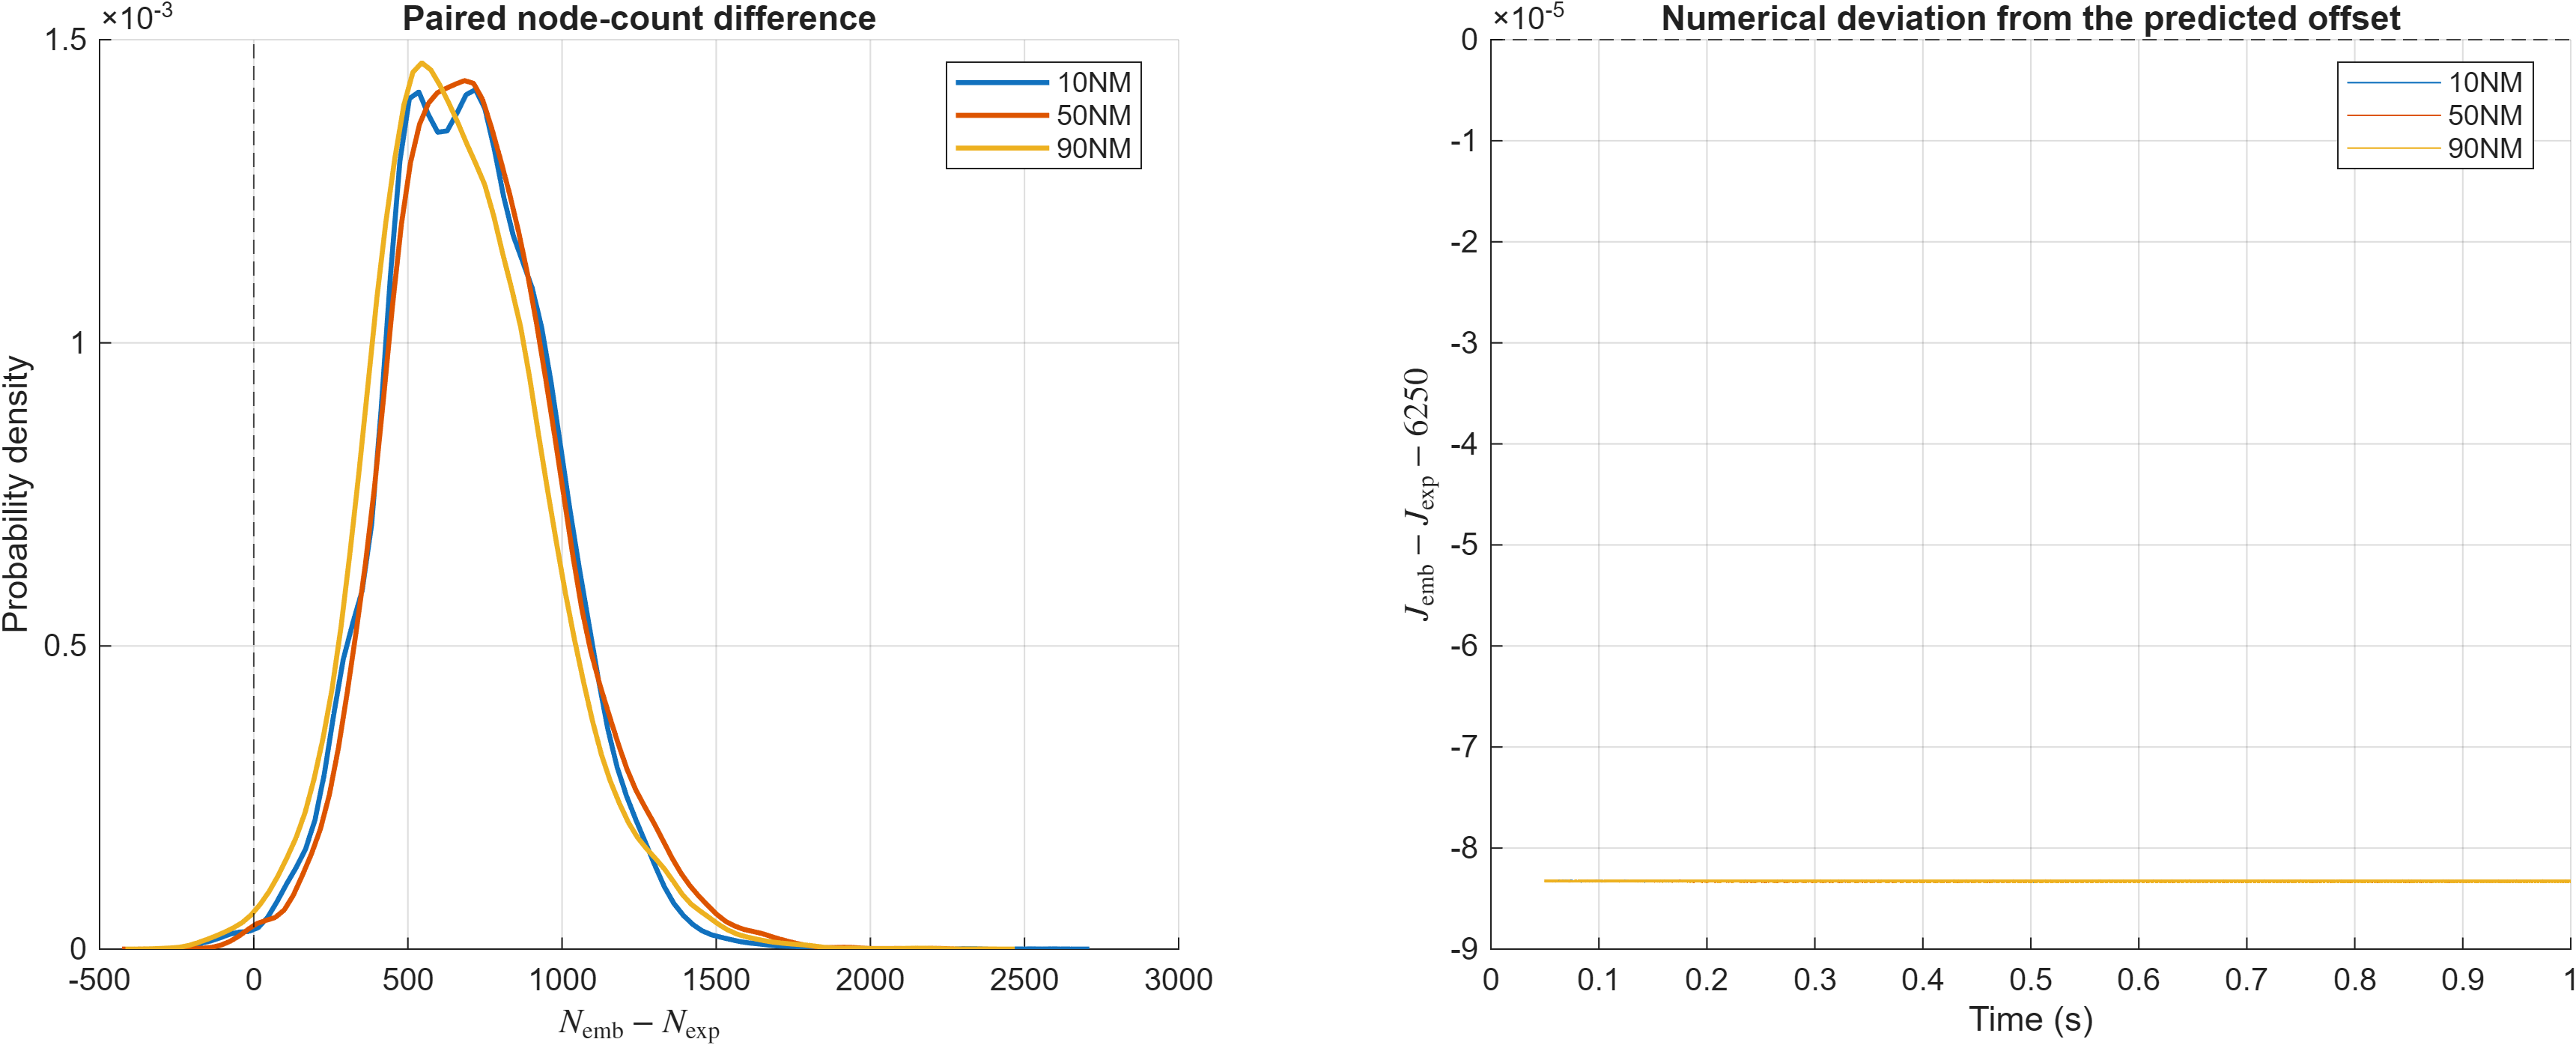
\includegraphics[width=\textwidth]{../figures/global_node_difference_and_cost_offset.png}
 \caption{Left: kernel-density estimate of the paired node-count difference
 $\Delta N=N_{\mathrm{emb}}-N_{\mathrm{exp}}$; positive values mean that the
 embedded solver visited more nodes.  The area below each curve equals one,
 whereas its height is a density rather than a point probability.  Right: numerical
 deviation of the measured leaf-cost difference from the predicted constant
 6250.}
 \label{fig:global_comparison}
\end{figure}

Independent replay of 500 uniformly distributed transactions per run produced
the mean node counts in \cref{tab:mean_nodes}.  Every replayed transaction
matched the logged optimum, node count, and switching sequence.
\begin{table}[H]
 \centering
 \caption{Mean visited nodes in the independently replayed sample.}
 \label{tab:mean_nodes}
 \begin{tabular}{lrrr}
 \toprule
 Torque & Embedded $H$ & Explicit penalty & Difference\\
 \midrule
 10~Nm & 1151.87 & 479.55 & 672.32\\
 50~Nm & 1177.64 & 474.69 & 702.95\\
 90~Nm & 1095.46 & 462.34 & 633.12\\
 \bottomrule
 \end{tabular}
\end{table}

\section{Depth-resolved behavior}
\begin{figure}[H]
 \centering
 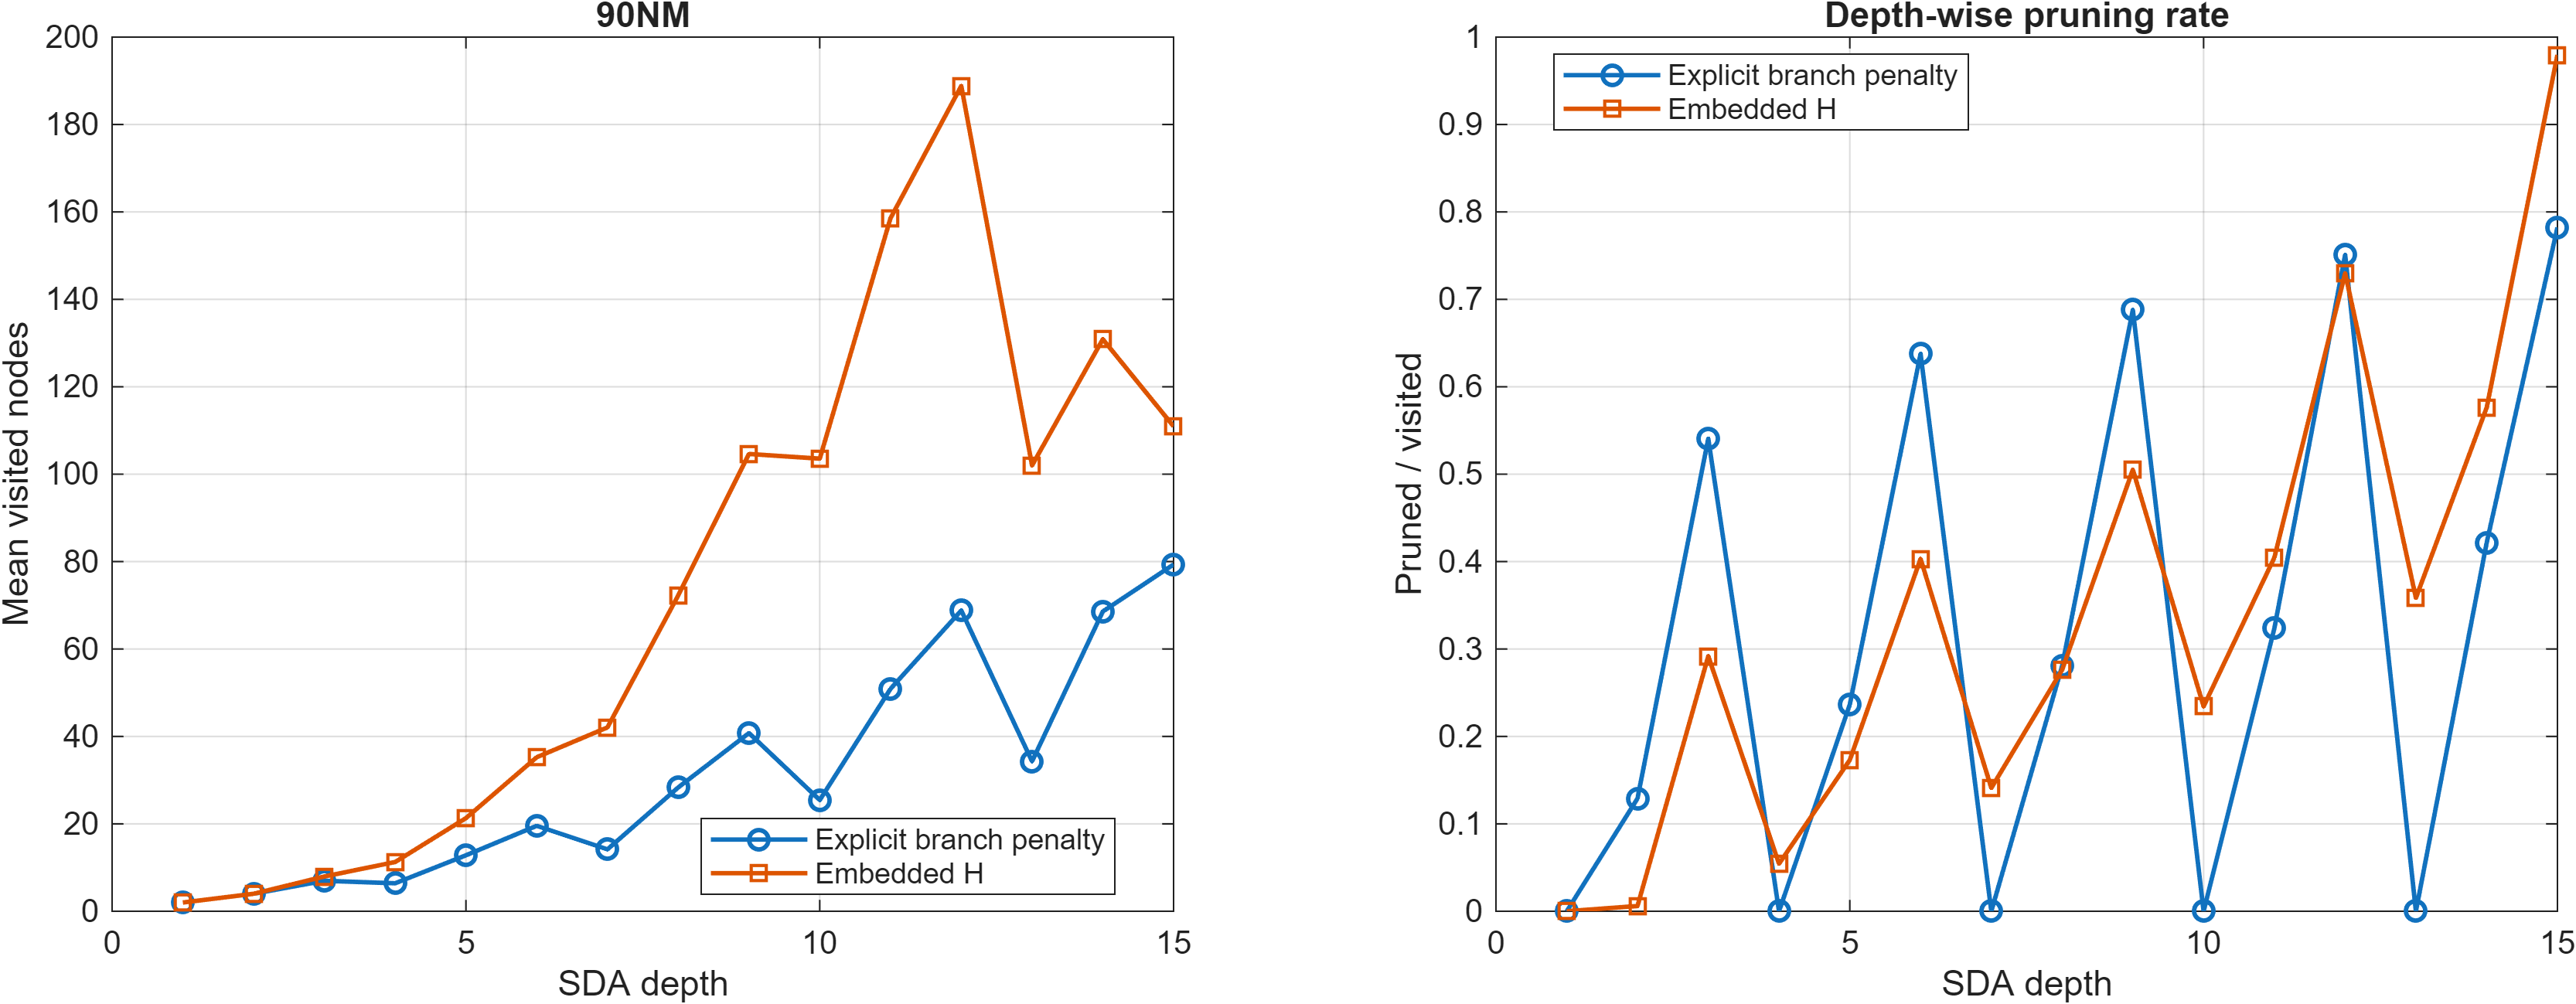
\includegraphics[width=\textwidth]{../figures/depth_statistics_90NM.png}
 \caption{Mean visited nodes and aggregate pruning rate versus search depth at
 90~Nm.  The explicit formulation exhibits pronounced pruning-rate peaks at
 several complete three-switch block boundaries, while the embedded
 formulation carries more surviving candidates into deeper levels.}
 \label{fig:depth90}
\end{figure}
The same qualitative behavior appears at 10 and 50~Nm.  This result supports
the block-boundary-alignment hypothesis, but does not yet prove that the 6250
offset is the sole cause.

\section{Representative median case}
At 90~Nm, the median node-difference case occurs at transaction 2305 and
$t=0.057625$~s.  The explicit search visits 494 nodes and the embedded search
1140 nodes, giving $\Delta N=646$.
\begin{figure}[H]
 \centering
 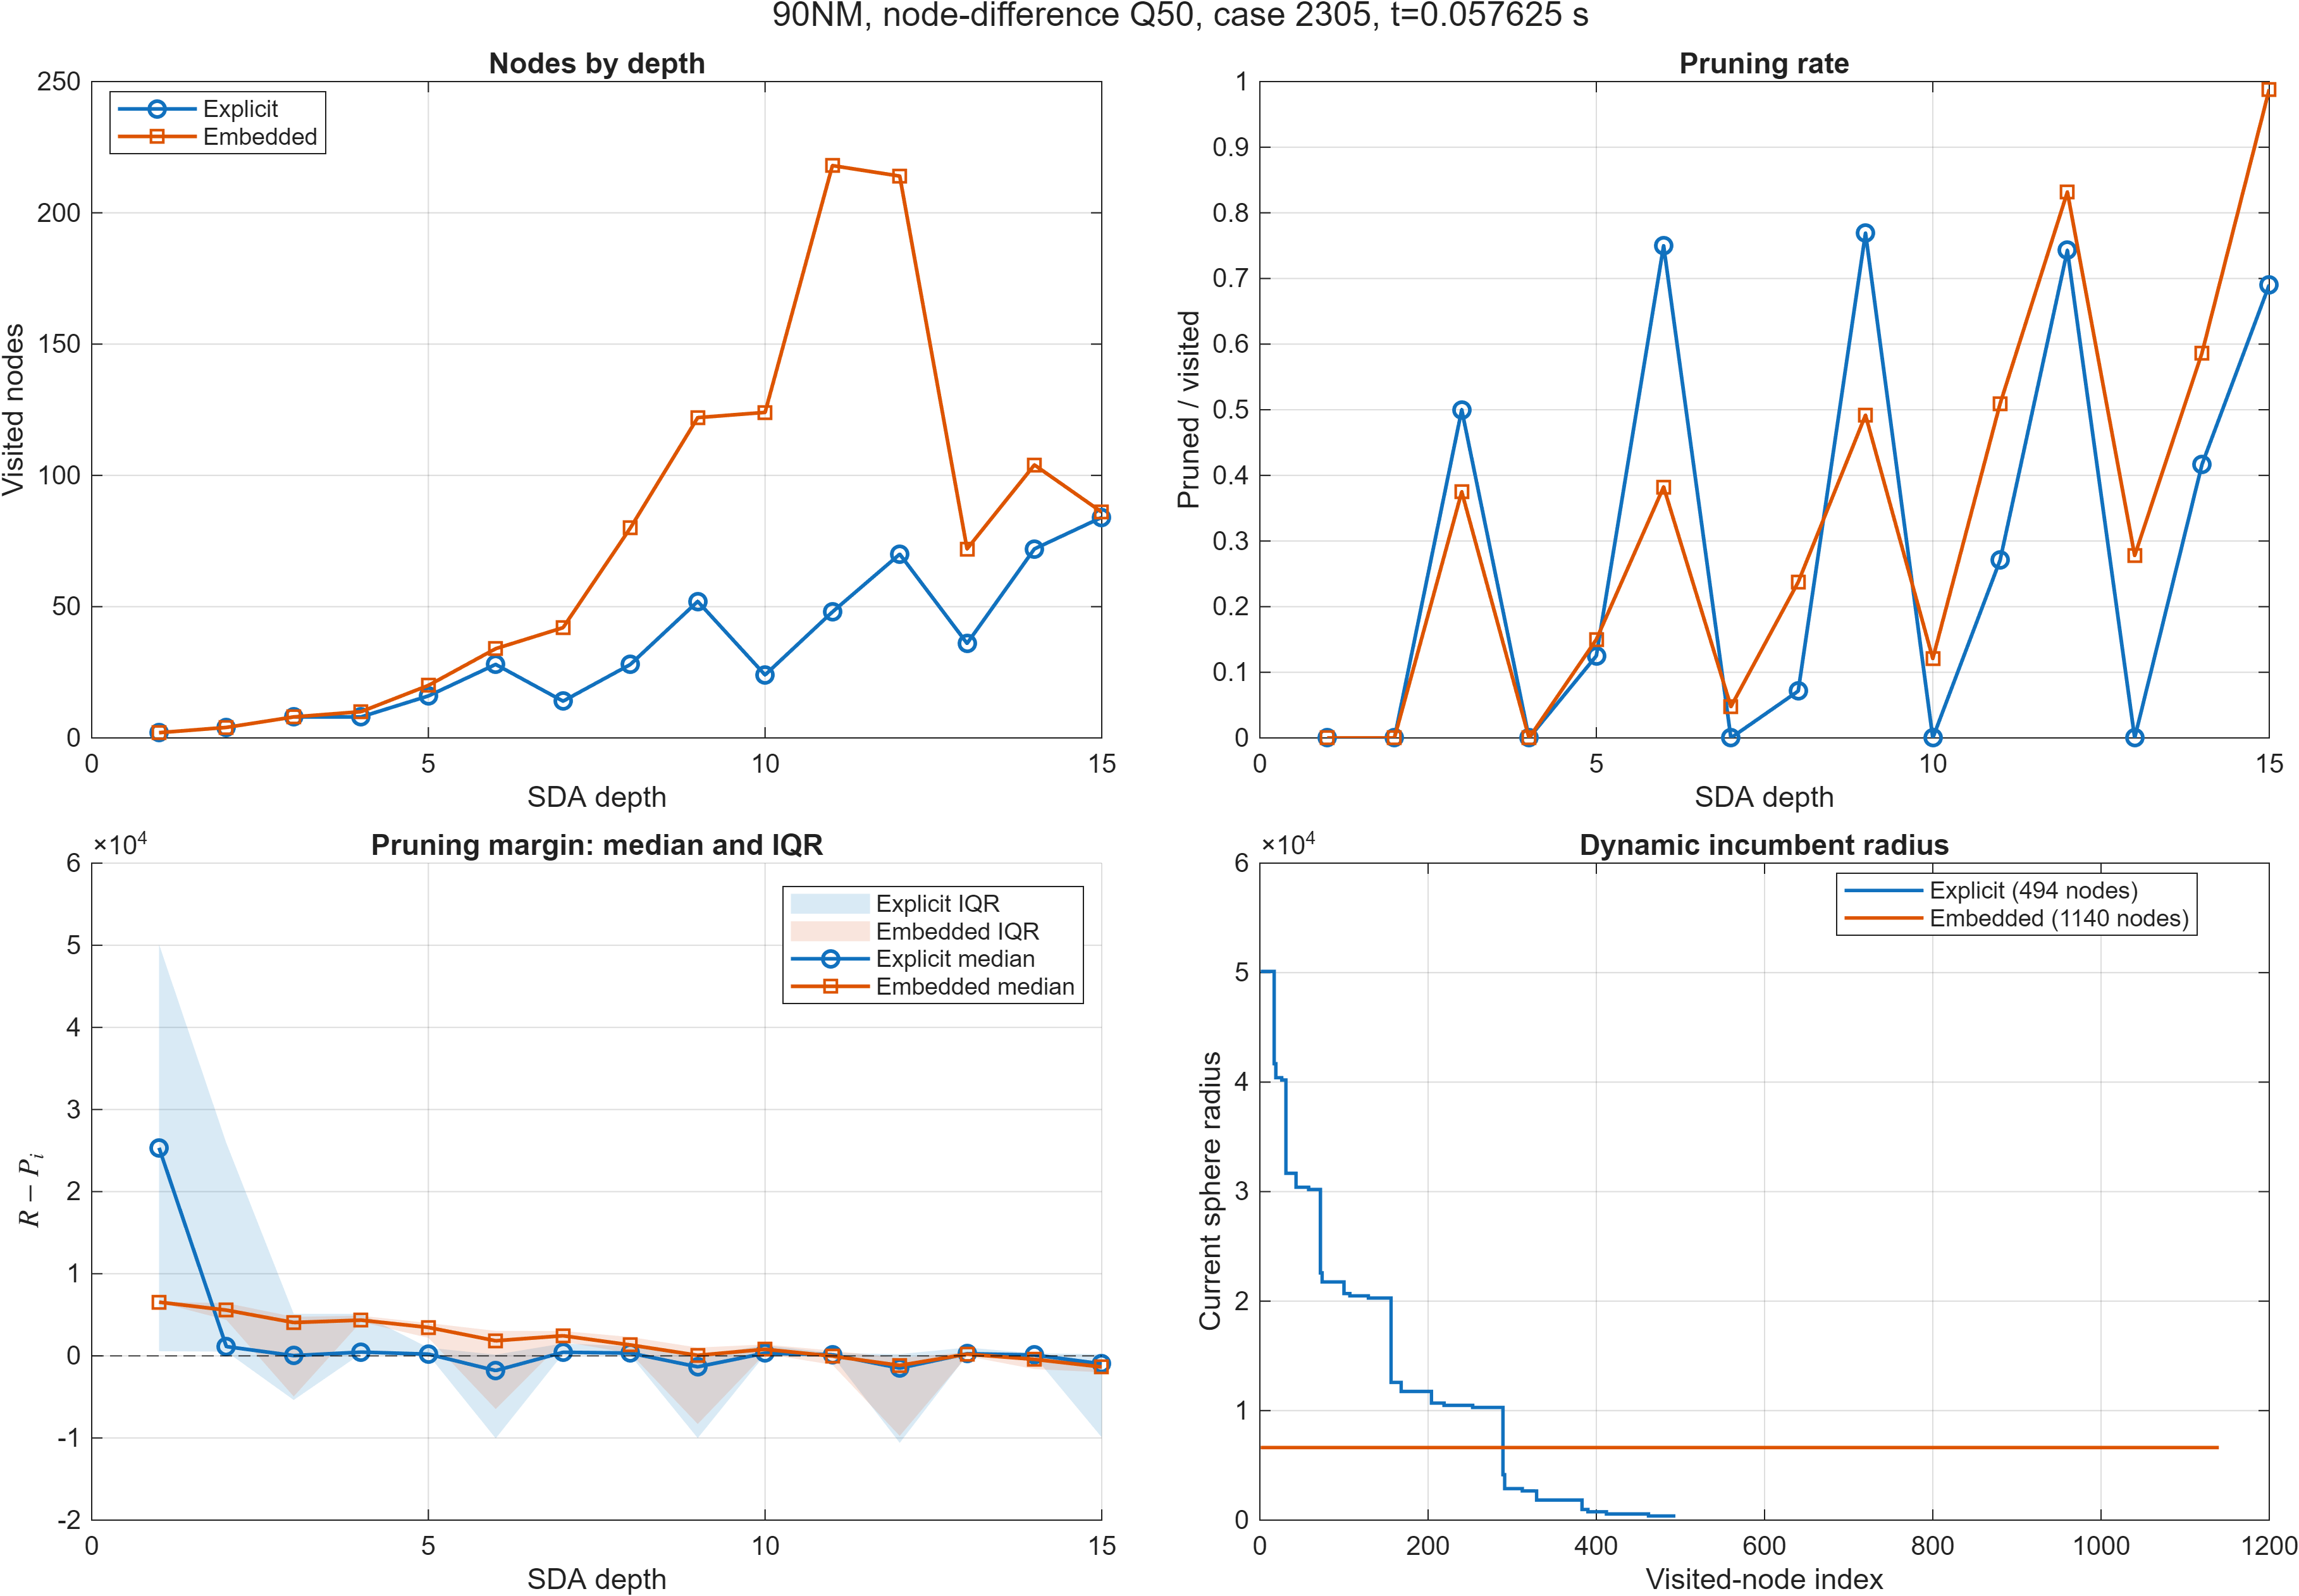
\includegraphics[width=\textwidth]{../figures/representative_90NM_Q50_case_2305.png}
 \caption{Search diagnostics for the 90~Nm median node-difference case.  The
 lower-left panel reports $M_i=R-P_i$ using the radius immediately before each
 tested node: positive values survive and negative values are pruned.  Solid
 lines are medians and shaded regions contain the middle 50\% of observations
 (IQR).  The lower-right panel shows how the best known complete cost, called
 the incumbent radius, changes with visited-node index.}
 \label{fig:representative90}
\end{figure}

The figure adds an important qualification to the initial hypothesis.  In this
case the embedded Babai incumbent is already close to its final value and its
radius remains almost constant.  The explicit formulation starts from a much
larger incumbent but discovers better leaves early and rapidly contracts its
radius.  The embedded solver nevertheless visits more nodes, especially at
intermediate depths.  Hence the raw initial-radius magnitude cannot by itself
explain the complexity difference.  The evidence instead points to the joint
effect of prefix-bound tightness, block-boundary penalties, enumeration order,
and dynamic incumbent updates.

\section{Representative-case definition}
The selected $(Q_5,Q_{50},Q_{95})$ node differences are respectively
$(282,692,1148)$ at 10~Nm, $(314,706,1226)$ at 50~Nm, and
$(244,646,1166)$ at 90~Nm.  All corresponding figures and exact transaction
indices are retained with the analysis data to prevent subjective figure
selection.

\section{Complete same-prefix enumeration}
The complete prefix tree was subsequently enumerated for all nine selected
transactions.  At depth $i$, all $2^i$ binary prefixes were evaluated under
both formulations.  This removes the ambiguity of comparing differently
ordered, actually visited nodes.  At every complete leaf and in every selected
case, the measured difference was
\begin{equation}
 P_{15}^{\mathrm{emb}}-P_{15}^{\mathrm{exp}}
 =6249.99992
\end{equation}
for all $2^{15}$ sequences; the tiny deviation from 6250 is numerical.

\begin{figure}[H]
 \centering
 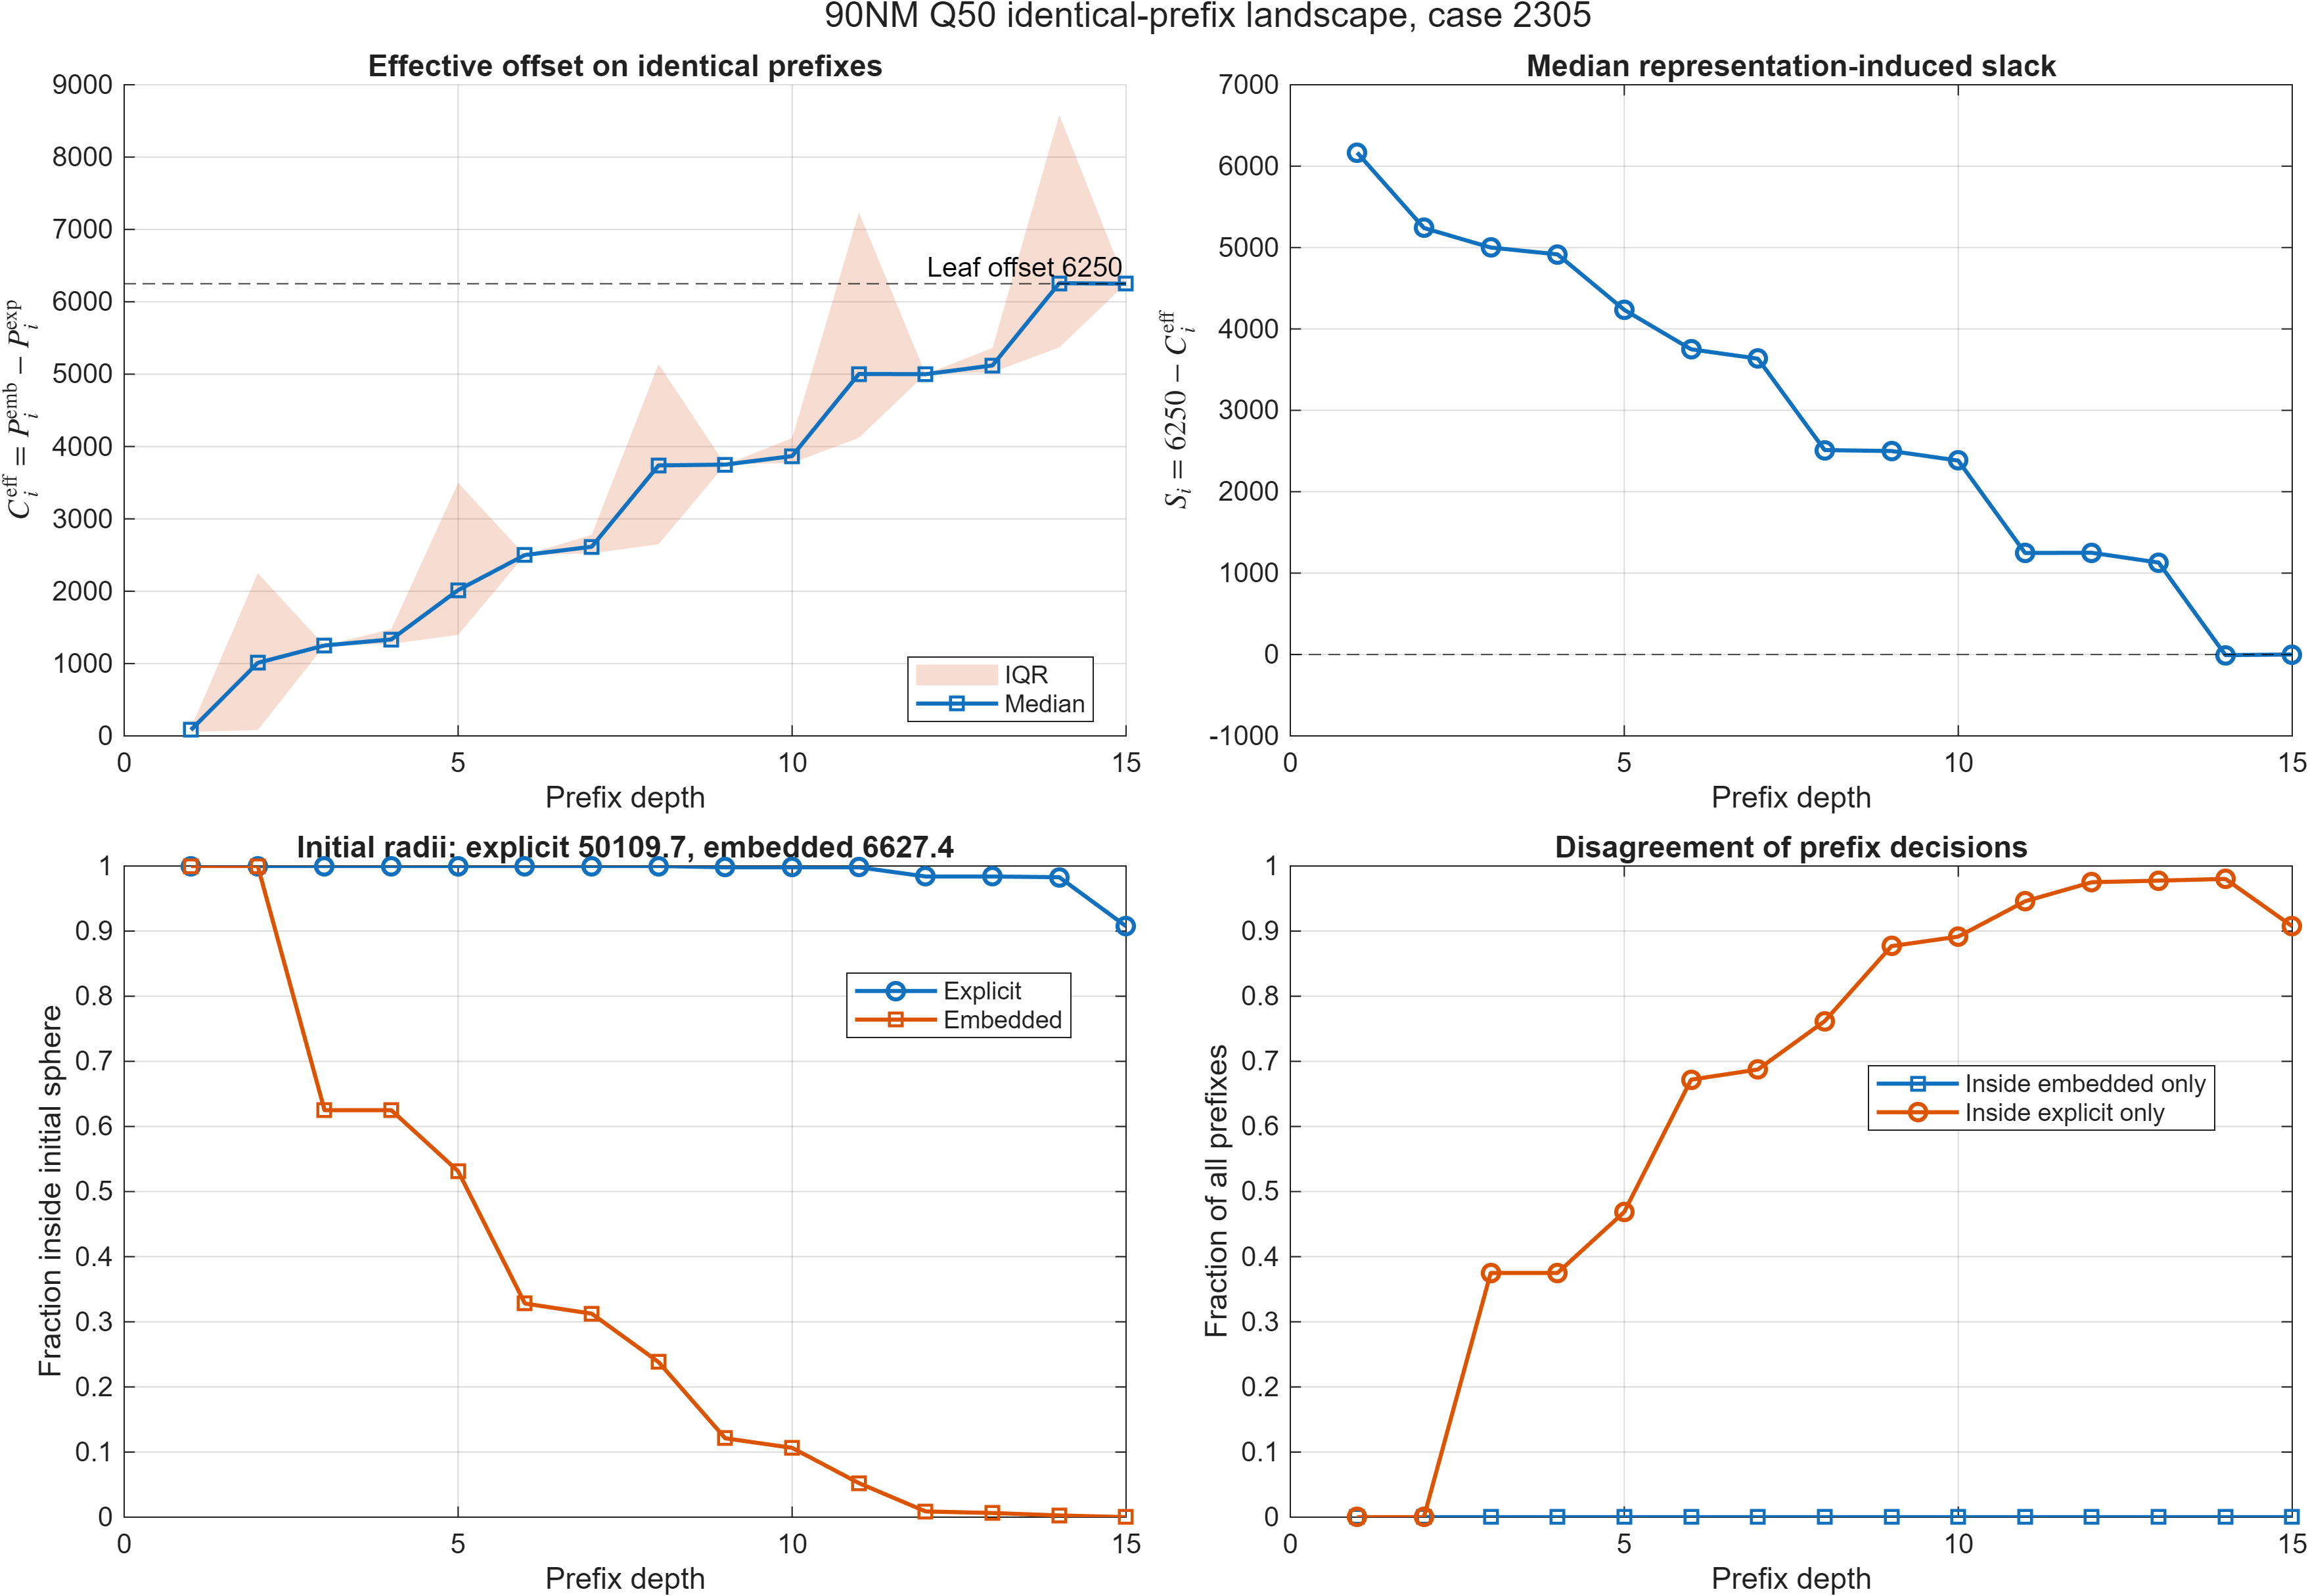
\includegraphics[width=\textwidth]{../figures/same_prefix/same_prefix_90NM_Q50_case_2305.png}
 \caption{Complete same-prefix landscape for the 90~Nm median case.  Top
 left: effective prefix offset and its interquartile range.  Top right:
 remaining median slack.  Bottom left: fraction of all prefixes inside each
 formulation's initial sphere.  Bottom right: prefixes classified inside only
 one of the two initial spheres.}
 \label{fig:sameprefix90}
\end{figure}

The median $C_i^{\mathrm{eff}}$ increases progressively toward 6250, and the
corresponding median $S_i$ decreases toward zero.  This confirms that the leaf
offset is not uniformly present in shallow partial metrics.  However, the
initial-radius comparison provides an important counterexample to a simple
``larger embedded sphere'' explanation.  In this transaction,
\begin{equation}
 R_{0,\mathrm{exp}}=50109.7,
 \qquad
 R_{0,\mathrm{emb}}=6627.4.
\end{equation}
The explicit initial sphere contains almost all prefixes through most depths,
whereas the embedded initial sphere is substantially tighter.  A static test
against the initial radii would therefore predict more aggressive embedded
pruning, opposite to the actually observed node count.

The discrepancy is resolved by recognizing that the initial sphere is not the
sphere used throughout the search.  As shown in
\cref{fig:representative90}, the explicit search discovers progressively
better leaves and rapidly reduces its incumbent radius.  The embedded Babai
incumbent begins near its final value and remains almost unchanged.  Actual
complexity is consequently determined by the coupled sequence
\begin{equation}
 \text{conditional centers}
 \rightarrow
 \text{enumeration order}
 \rightarrow
 \text{time of first good leaves}
 \rightarrow
 \text{dynamic radius contraction}
 \rightarrow
 \text{later pruning decisions},
\end{equation}
in addition to the depth distribution of the zero-vector cost.

\section{Hybrid and oracle ablation results}
The five configurations were replayed on 500 transactions per torque
condition.  All configurations returned the logged globally optimal switching
sequence.  \Cref{tab:hybrid_nodes} reports the total node count.

\begin{table}[H]
 \centering
 \caption{Ablation of initialization and search representation.  Entries are
 mean visited nodes; values in parentheses are the 95th percentiles.}
 \label{tab:hybrid_nodes}
 \begin{tabular}{lrrr}
 \toprule
 Method & 10~Nm & 50~Nm & 90~Nm\\
 \midrule
 Native explicit & 451.96 (919) & 466.67 (1033) & 442.48 (867)\\
 Native embedded & 1140.90 (1794) & 1179.00 (1845) & 1100.20 (1745)\\
 Hybrid & \textbf{182.66 (489)} & \textbf{191.49 (500)} & \textbf{199.92 (504)}\\
 Oracle explicit & 160.49 (427) & 161.12 (380) & 150.97 (313)\\
 Oracle embedded & 1123.00 (1746) & 1137.90 (1808) & 1010.40 (1662)\\
 \bottomrule
 \end{tabular}
\end{table}

Relative to the native explicit solver, the hybrid reduces the mean node count
by 59.6\%, 59.0\%, and 54.8\% at 10, 50, and 90~Nm, respectively.  Relative
to the native embedded solver, the corresponding reductions are 84.0\%,
83.8\%, and 81.8\%.  Its mean node count lies close to the unattainable oracle
explicit baseline, which supplies the true optimum before search begins.

\begin{figure}[H]
 \centering
 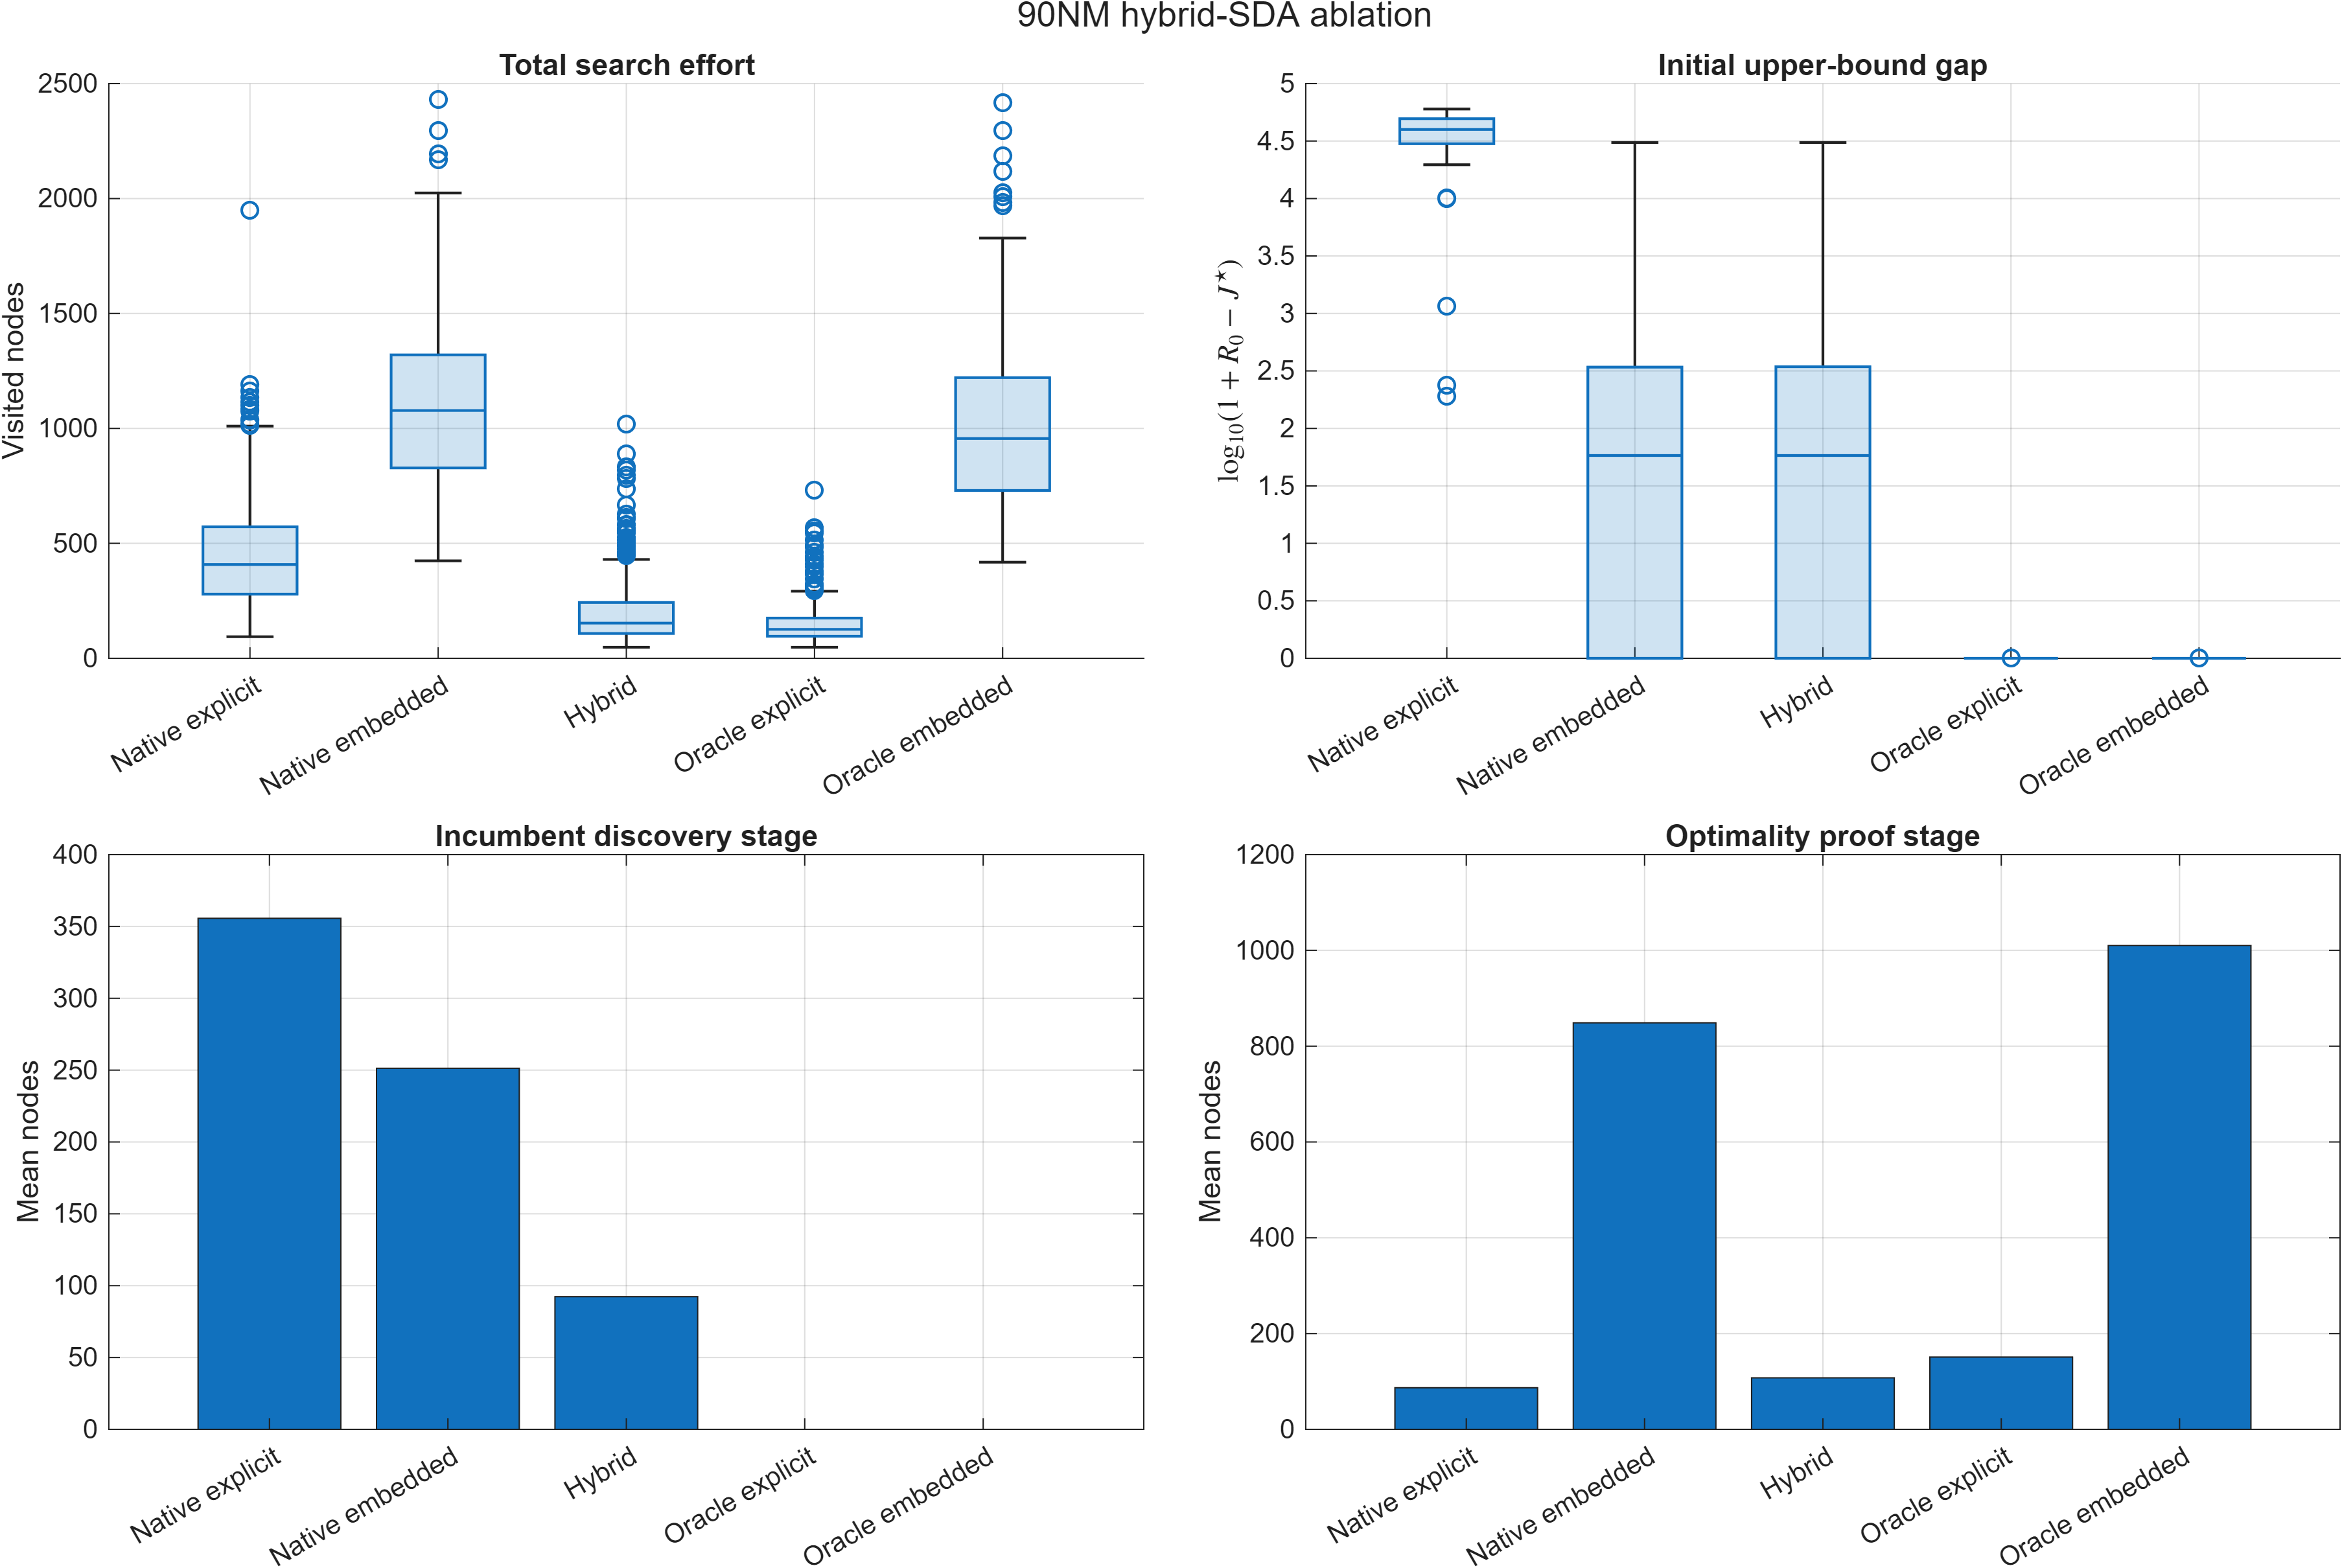
\includegraphics[width=\textwidth]{../hybrid_results/hybrid_ablation_90NM.png}
 \caption{Hybrid-SDA ablation at 90~Nm.  The upper-left panel compares total
 visited nodes.  The upper-right panel reports the initial upper-bound gap on a
 logarithmic display.  The lower panels partition the trace at the first
 occurrence of the known optimum.  Oracle configurations isolate the search
 representation by supplying the optimum at node zero.}
 \label{fig:hybrid90}
\end{figure}

\subsection{Evidence for the embedded upper-bound advantage}
The native explicit initializer was not optimal in any of the 1500 sampled
transactions.  Its median initial optimality gap was approximately 49279,
39947, and 39879 at 10, 50, and 90~Nm.  The embedded Babai sequence was already
optimal in 51.8\%, 49.2\%, and 40.0\% of the respective cases, with median gaps
of approximately zero, 2.55, and 57.12.  The hybrid inherits exactly this
sequence quality because it uses the embedded Babai point and merely
reevaluates it under the constant-shift-equivalent explicit objective.

These results support an empirical, not universal, claim: for the investigated
machine states, weight, horizon, and variable ordering, embedding the
zero-vector objective strongly improves the initial feasible upper bound.

\subsection{Evidence for the explicit proof advantage}
The oracle comparison supplies the optimal sequence to both searches and
therefore eliminates initializer quality as an explanation.  Even under this
condition, the explicit solver requires only 150.97--161.12 mean nodes, whereas
the embedded solver requires 1010.40--1137.90.  Thus, the explicit search uses
approximately 84--86\% fewer nodes to certify the same known optimum.

Together with \cref{eq:bound_advantage} and the depth-wise pruning peaks, the
oracle result provides strong evidence that the explicit formulation offers a
more effective branch-and-bound representation.  It does not prove universal
node dominance for every state or variable ordering, because intermediate
non-block depths remain path dependent.

\subsection{Interpretation of the hybrid improvement}
The hybrid combines two complementary properties rather than averaging two
controllers.  Its embedded Babai step lowers the initial upper-bound gap.  Its
explicit search retains the block-aligned lower bounds and rapidly certifies or
improves that incumbent.  The measured reduction is therefore consistent with
the intended chain
\begin{equation}
 \text{embedded upper bound}
 \;\longrightarrow\;
 \text{explicit prefix pruning}
 \;\longrightarrow\;
 \text{lower total search effort}.
\end{equation}
Because the Babai sequence is reevaluated under the explicit objective and the
subsequent solver is unchanged, the node reduction does not trade away control
optimality.

\chapter{Remaining Analysis}

The current results prove leaf equivalence, establish a repeatable complexity
difference, and complete the same-prefix comparison of
$P_i^{\mathrm{exp}}$, $P_i^{\mathrm{emb}}$, $C_i^{\mathrm{eff}}$, $S_i$, and
initial-sphere membership.  They also reject the hypothesis that a larger
embedded initial radius is by itself responsible for the additional nodes.

The hybrid and oracle experiments now separate initializer quality from search
representation at the node-count level.  Before integration into the final
thesis, three engineering questions remain.  First, execution time rather than
node count must be measured, including the additional embedded factor and
Babai pass.  Second, memory and 10~kHz precomputation cost must be reported.
Third, worst-case and high-percentile execution times must be compared with the
available real-time deadline.

A further theoretical refinement would compute, for every prefix, the exact
best achievable completion cost
\begin{equation}
 L_i^\star(\vct U_{1:i})
 =\min_{\vct U_{i+1:n}}J(\vct U)
\end{equation}
and the lower-bound slack
\begin{equation}
 \Gamma_i=L_i^\star-P_i.
\end{equation}
The finite 15-bit search space makes this exhaustive offline calculation
possible.  It would quantify bound tightness independently of traversal order,
but it is not required for the already established correctness of the hybrid
solver.

The refined causal chain to test is
\begin{equation}
 \text{quadratic representation and conditional centers}
 \Longrightarrow
 \text{different enumeration order and leaf discovery time}
 \Longrightarrow
 \text{different dynamic-radius history}
 \Longrightarrow
 \text{more visited nodes}.
\end{equation}
The block-boundary penalty and nonuniform prefix offset remain contributing
mechanisms, but the evidence no longer supports attributing the observed node
difference to the raw initial-radius magnitude alone.

\chapter{Reproducibility Assets}
The analysis source, extracted data, validation outputs, representative-case
selection, and generated figures are maintained under
\texttt{Model\_2025b/SDA\_embedded\_analyze}.  The production Simulink model and
production SDA source are not modified by the profiling workflow.

\end{document}
